%Paqueterias
\documentclass[12pt,letterpaper,final]{article}%Tipo de documento
\usepackage[utf8]{inputenc}
\usepackage[spanish,es-nodecimaldot]{babel}
\usepackage{amsmath}
\usepackage{amssymb}
\usepackage{graphicx}
\usepackage[left=2cm,right=2cm,top=2cm,bottom=2cm]{geometry}
\usepackage{titlesec}
\usepackage{hyperref}
\usepackage{pdflscape}
\usepackage{gensymb}
\usepackage{stix2}
\usepackage{siunitx}
\graphicspath{{images/}}
\baselinestretch
\renewcommand{\baselinestretch}{1.25}%Comando de interlineado
%%%%%%%%%%%%%%%%%%%%%
\usepackage{fancyhdr}%Encabezados
\pagestyle{fancy}
\fancyhf{}
\lhead[\leftmark]{Reporte semestral}
\rhead[]{\rightmark}
\lfoot[\thepage]{}
\rfoot[]{\thepage}
\renewcommand{\headrulewidth}{0.5pt}
\renewcommand{\footrulewidth}{0pt}
\fancypagestyle{plain}{
	\fancyhead[L]{Omar Arturo Castillo M\'endez}
	\fancyfoot[R]{\thepage}
	\renewcommand{\headrulewidth}{0.4pt}
	\renewcommand{\footrulewidth}{0.4pt}
}
\pagestyle{fancy}
%%%%%%%%%%%%%%%%%%%%%%%%%
%Datos del documento
\title{Reporte de final de primer semestre}
\date{}
\author{M.I.E. Omar Arturo Castillo M\'endez}
\begin{document}
	%%%%%%%%%%%%%%%%%%%%%%%%%%%%%%%%%%%%%%%%%%%%%%%%%%%%%
	\begin{titlepage}%Portada
		\centering
		
\includegraphics[scale=1]{logo}
		\vspace{0.1cm}
		{\bfseries\LARGE Tecnol\'ogico Nacional de M\'exico \par}
		{\bfseries\LARGE Centro Nacional de Investigaci\'on y Desarrollo Tecnol\'ogico \par}
		\vspace{0.25cm}
		{\scshape\Large Departamento de Ciencias en Ingenier\'ia Electr\'onica \par}
		\vspace{0.25cm}
		{\scshape\Large Diseño, construcci\'on y puesta en marcha de un regenerador de energ\'ia para el desarrollo y la validaci\'on de estrategias de modelado matem\'atico \par}
		\vspace{0.25cm}
		{\itshape\Large Reporte de quinto semestre  \par}
		\vspace{0.25cm}
		{\bfseries Director de tesis: \par}
		\vspace{0.2cm}
		{Dr. V\'ictor Manuel Alvarado Mart\'inez \par}
		\vspace{0.2cm}
		{\bfseries Co-Directora de tesis: \par}
		\vspace{0.2cm}
		{Dra. Ma. Guadalupe L\'opez L\'opez \par}
		\vspace{0.2cm}
		{\bfseries Comit\'e revisor: \par}
		\vspace{0.2cm}
		{Dr. Jos\'e Francisco G\'omez Aguilar \par}
		\vspace{0.2cm}
		{Dr. Ricardo Fabricio Escobar Jim\'enez  \par}
		\vspace{0.2cm}
		{Dr. Jarniel Garc\'ia Morales \par}
		\vspace{0.2cm}
		{\bfseries Presenta: \par}
		{M.I.E. Omar Arturo Castillo M\'endez \par}
		\vspace{0.2cm}
		{\today \par}
	\end{titlepage}
	%%%%%%%%%%%%%%%%%%%%%%%%%%%%%%%%%%%%%%%%%%%%%%%%%%%%%%%
	\tableofcontents{\thispagestyle{empty}}
	%\tableofcontents{\thispagestyle{empty}} Pagina sin numeracion
	\newpage
	%\listoffigures{\thispagestyle{empty}}
	%\newpage
	\setcounter{page}{1}

\section{Introduci\'on}
Este reporte presenta una revisión de algunos modelos de regeneradores de lecho empacado, un componente fundamental en diversos procesos industriales como la separación de gases, la purificación de líquidos y la recuperación de calor. Ademas, presentar una versión de un modelo de regenerador, así como la obtención de los parámetros que son necesarios para el desarrollo del mismo considerando aspectos físicos: las propiedades térmicas de la fase solida y gaseosa, del gas como el numero de Reynolds, porosidad del lecho, etc.

\section{Revisión del estado del arte}
En esta sección, se describen trabajos que son importantes para el desarrollo del modelado, ademas para revisar cuales son las diferencias entre modelos que tienen una estructura similar, que parámetros se están considerando para su solución, suposiciones de modelado, condiciones de frontera. Para tener una perspectiva mas amplia de como estas características funcionan para simplificar o aumentar su dificultar para obtener una solución. A continuacion se presenta cada trabajo, por su titulo original y se describe el modelo utilizado, consideraciones, condiciones iniciales y de frontera. 
\subsection*{Modeling a heat regenerator-reactor with temperature dependent gas properties}
La principal característica de los regeneradores de energía, es que en el mismo espacio de manera alternada puede contener dos gases. En el espacio vacío del regenerador, el gas mas caliente fluye y cede su energía térmica a las partes solidas (debe tener una alta capacidad y densidad térmica), posteriormente un gas frío recupera ese calor durante un intervalo de tiempo. Para este trabajo, se consideró como constante el coeficiente de transferencia de calor, pero tomó como variable la compresibilidad del gas. Se modeló asumiendo un sistema adiabático, la conductividad térmica del solido infinitamente normal al flujo del gas y cero paralelo al flujo, conexión ideal del gas, asumiendo que no existe dispersión del gas en las conexiones. El modelo se dividió en tres ecuaciones usando balances de energía y masa tradicionales, el sistema se considero cerrado a la entrada, las variaciones de la velocidad al inicio del regenerador no afecta sus condiciones de entrada, existe una pequeña acumulación de masa en el regenerador antes o después de completar el cambio de temperaturas. Para el periodo de calentamiento, la velocidad del gas incrementa y la densidad disminuye(disminución neta de masa). El balance del gas en cualquier posición axial, parte de \textit{la suma de razón de entalpía de entrada , la razón de salida y la transferida resulta en la razón de acumulación de la entalpía}\cite{Kulkarni1992} 
\begin{equation}
	\frac{\partial T_g}{\partial t} = -\frac{1}{\epsilon L}[u\frac{\partial T_g}{\partial z}+ \frac{ha_p L}{\rho u C_p}(T_g-T_s)]
\end{equation}
Donde $u$ es la velocidad del gas en $\frac{m}{s}$, $\epsilon$ es la porosidad del regenerador
\newline
El balance de energía correspondiente al solido:
\begin{equation}
	\frac{dT_s}{dt} = \frac{ha_p}{(1-\epsilon)\rho_s C_{ps}}(T_g-T_s)
\end{equation}
El balance de masa:
\begin{equation}
	\frac{du}{dz} = -\frac{Rha_pL}{PM_wC_p}(T_g-T_s)
\end{equation}
En el balance de masa se esta considerando z como adimensional $z=\frac{x}{L}$
\newline
Las condiciones iniciales y de frontera:
\begin{equation*}
	T_g(0,z)=T_{g \,inicial} \quad T_g(t,0)=T_{g \,entrada} \quad T_s(0,z)= T_{s \, inicial} \quad u(t,0) = u_{entrada}
\end{equation*}
\subsubsection*{Parámetros del modelo}
La ley de los gases ideales:
\begin{equation}
	PV=N_m R T
\end{equation}
Donde: $N_m$ numero total de moles de cualquier gas, $R$ constante de los gases ideales y $T$ la temperatura del gas.
\begin{equation}
	a_p=\frac{6(1-\epsilon)}{d_p}
\end{equation}
Donde $a_p$ corresponde a la superficie especifica en el empaquetado, $d_p$ es el diámetro del relleno y $\epsilon$ a la porosidad del regenerador. 
\newline
La capacidad calorífica se puede obtener mediante la siguiente expresión, solo considerando que cambia conforme la variación de temperatura del gas\cite{green2018perry}, en caso contrario se puede considerar como constante:
\begin{equation}
	C_p=(0.79)[6.5+0.001(T_g)] + (0.21)(8.27+0.000258(T_g)-\frac{187700}{T_g^2}) \quad \frac{cal}{mol\cdot s \cdot K}
	\end{equation}
Las correlaciones semi-empiricas para el coeficiente de transferencia de calor pueden obtenerse mediante las siguientes expresiones\cite{Levenspiel1983}:
\begin{equation}
	Nu = 2 - 1.8 Re^{\frac{1}{2}}Pr^{\frac{1}{3}}
\end{equation}
\begin{equation*}
	Nu = \frac{hd_p}{k_g} \quad Re = \frac{d_p u\rho}{\mu} \quad Pr=\frac{C_p \mu }{k_g}
\end{equation*}

\subsection*{Solution by triple collocation for periodic operation of heat regenerators}

El método basado en colocación triple ha sido desarrollado para simulación de regeneradores de energía mediante un modelo lineal. El problema se reduce a un conjunto de ecuaciones algebraicas lineales. El problema del valor inicial en un regenerador al arranque y durante su operación puede ser resuelto por este método para cualquier modelo de ecuaciones. 
\newline
Los regeneradores de calor son usados de manera extensa en procesos industriales donde el gas se encuentra disponible a temperaturas altas y bajas. Algunos ejemplos importantes, recuperación de calor en centrales termoeléctricas, pre-calentamiento de aire, recuperación de calor de los gases de desperdicio en la fundición del hierro,en la manufacturación del vidrio, almacenamiento de energía solar, etc \cite{Ramachadran1984}.
\newline
\subsubsection*{Ecuaciones del modelo}
Las ecuaciones del modelo en su forma adimensional describen un empaquetado de un regenerador con la siguiente forma:
\newline
La primera ecuación representa un balance de energía, como es el cambio de temperatura entre la fase solida y el gas.
\begin{equation}
	\frac{1}{Pe}\frac{\partial ^2 \theta_h}{\partial x^2} - \frac{\partial \theta_h}{\partial x} - St(\theta_h -\theta_{phs}) = 0
\end{equation}
La siguiente corresponde a un balance de energía para indicar la temperatura de la partícula:
\begin{equation}
	\frac{1}{y^2}\frac{\partial}{\partial y}(y^2\frac{\partial \theta_{ph}}{\partial y}) = \frac{\partial \theta_{ph}}{\partial t} 
\end{equation}
La dirección en $x$ y $y$ son para referirse a la posición axial adimensional dentro del regenerador y a la forma esférica de la partícula respectivamente. $\theta_h$ es la temperatura de la masa del gas dentro del regenerador durante el periodo de calentamiento, para una posición en $x$ y un tiempo $t$. $\theta_{ph}$ es la temperatura de la partícula durante el periodo de calentamiento para una posición $x$ dentro del regenerador y una posición radial en $y$ en el tiempo. Finalmente, $\theta_{phs}=\theta_{ph}(x,y=1,t)$ es la temperatura externa de la superficie de la esfera.
\newline
Las condiciones de frontera son:
\begin{equation}
	x = 0, \qquad \frac{1}{Pe}\frac{\partial \theta_h}{\partial x} = \theta_h - \theta_{h,en}
\end{equation} 
\begin{equation}
	x = 1, \qquad \frac{\partial \theta_h}{\partial x} = 0
\end{equation}
\begin{equation}
	x = 0, \qquad \frac{\partial \theta_{ph}}{\partial y} = 0
\end{equation} 
\begin{equation}
	x = 1, \qquad \frac{1}{Bi}\frac{\partial \theta_{ph}}{\partial y} = \theta_h - \theta_{phs}
\end{equation}
Donde $\theta_{h,en}$ es la entrada adimensional de la temperatura del gas caliente. La ecuaciones y condiciones de frontera están basadas según la suposición, la transferencia de energía ocurre mediante flujo másico, la dispersión es axial en la fase gaseosa, la transferencia entre fluido, partículas y su parte interna es por conducción, no se consideró la transferencia de calor por radiación y conducción entre partículas. Las propiedades físicas y parámetros de transporte se asumen independientes de la temperatura. La condición inicial para la parte interna de las partículas es la siguiente:
\begin{equation}
	t=0, \qquad \theta_{ph} = \theta_{ph0}(y,x)
\end{equation}
El valor de $\theta_{ph0}$ representa la temperatura inicial que se distribuye para el periodo de enfriamiento y la temperatura de distribución al final del periodo de calentamiento, si solo se considera un solo ciclo el valor $\theta_{ph0}=0$.
\newline
\subsubsection*{Números adimensionales}
\begin{itemize}
	\item Número de Stanton [St] = $\frac{h a_p L}{u_g \rho_g C_{pg}}$
	\item Número de Biot [Bi] = $\frac{h R}{\lambda_e}$
	\item Número de Peclet [Pe] = $\frac{ u_g \rho_g C_{pg} L}{\lambda_{ax}}$
	\item Tiempo adimensional [t] = $\frac{t_a \lambda_e}{\rho_s C_{ps} R^2}$ o $ \frac{h a_p t_a }{(1-\epsilon_B)\rho_s C_{ps}} = 3 (Bi) t $
	
\end{itemize}

\subsection*{Mathematical models for the simulation of thermal regenerators:
	A state-of-the-art review}
Los regeneradores de lecho fijo pueden estar identificados por dos tipos: rotatorios o de lecho fijo. En un lecho fijo el regenerador almacena materiales que son fijos dentro, y el uso de válvulas solenoides permiten el paso de gas caliente o frío de manera alternada. Liberando su calor al lecho durante el periodo de calentamiento, posteriormente un flujo frío absorbe ese calor que ganó el lecho durante el calentamiento, y esto corresponde al periodo de enfriamiento. Es común el uso de materiales como: aluminio, acero, vidrio para el armado del lecho\cite{SADRAMELI2016}.
\newline
El modelo esta basado según las siguientes consideraciones:
\begin{itemize}
	\item Las propiedades térmicas y físicas del gas y el solido son constantes e independientes de la temperatura y posición.
	\item No existe perdida de calor del regenerador hacia el ambiente.
	\item No hay fuentes de energía que ocurran dentro del regenerador ni reacciones químicas internas
	\item La capacidad térmica del gas dentro del lecho en cualquier instante es pequeña comparada con el lecho mismo.
	\item Los coeficientes de flujo másico y de transferencia de calor son constantes
	\item La velocidad de entrada y la temperatura para cada fluidos son uniformes a través de la sección transversal y constantes en el tiempo
	\item La conductividad térmica del solido es infinitamente mas grande en la dirección normal al flujo del gas e infinitamente pequeña en la dirección paralela del flujo.
	\item No existe dispersión de flujo dentro del regenerador.
	\item La transferencia de calor del fluido es insignificante longitudinal y transversalmente.
	\item El espacio vacío y la superficie de contacto del lecho son uniformes.
	\item El tiempo de residencia del gas dentro del lecho es insignificante en comparación al periodo.
	\item La transferencia de calor por radiación es pequeña en comparación con otros mecanismos de transferencia.
\end{itemize}
\subsubsection*{Modelo}
El modelo para un regenerador de lecho fijo, para la fase solida:
\begin{equation}
	M_s C_{ps}\frac{\partial T_s}{\partial \theta} = h a (T - t_h)
\end{equation}
Para la fase del fluido:
\begin{equation}
	\frac{G C_{pg}}{u}\frac{\partial t_h}{\partial \theta} + G C_{pg}\frac{\partial t_h}{\partial x} = ha(T_s - t_g)
\end{equation}
Las condiciones iniciales y de equilibrio del proceso son:
\begin{equation*}
	t_h(0,t_h) = t_{h,i} = cte , \qquad 0<t_h<P_h
\end{equation*}

\begin{equation*}
	t_h(0,t_c) = t_{c,i} = cte , \qquad 0<t_c<P_c
\end{equation*}
Para las condiciones de equilibrio:
\begin{equation*}
	T_{s,h}(x,t_h=0) = T_{s,c}(x,t_c=P_c)
\end{equation*}
\begin{equation*}
	T_{s,h}(x,t_h=0) = T_{s,c}(x,t_c=P_c)
\end{equation*}
\begin{equation*}
	0<x<L
\end{equation*}
Se resolvió el modelo redefiniendo los parámetros de longitud, temperatura y tiempo de manera unidimensional:
\begin{equation*}
	y = \frac{x}{L}
\end{equation*}
\begin{equation*}
	z_1 = \frac{(t-\frac{x}{u_1})}{P_1}
\end{equation*}
\begin{equation*}
	z_2 = \frac{(t-\frac{x}{u_2})}{P_2}
\end{equation*}
\subsection*{Review of Design and Modeling of Regenerative
	Heat Exchangers}
	Los regeneradores de energía, son dispositivos que usan de manera indirecta el intercambio de energía con medios fríos y calientes. El uso principal se encuentra en el área de la metalurgia, el tratamiento y pre-calentamiento del aire, recuperación del calor residual y en turbinas. En este trabajo se aplico el método abierto de Willmott, que mostró una gran estabilidad y permitieron la inclusión de ecuaciones que describen la transferencia de calor y la caída de presión. La ventaja de los regeneradores sobre los recuperadores es por su mayor área de contacto con relación a su capacidad volumétrica. Varios materiales y formas pueden usarse como material de relleno en el regenerador, porque los sólidos tienen una gran capacidad calorífica en comparación con los gases. Para pequeños regeneradores pueden usarse rellenos como los de panal de abeja, esferas, monolitos, anillos, monturas, etc.  \cite{Kilkovsky2020}
\subsubsection*{Modelo}
\begin{equation}
	M_b C_{p,b}\frac{\partial T_b}{\partial t} = h_t A (T_g - T_b) 
\end{equation}
Donde $M_b$ es la masa del relleno ($kg$), $T_b$ es la temperatura media del relleno ($^\circ C$), $h_t$ es el coeficiente global de transferencia de calor $(\frac{W}{m^2 K})$, $C_{p,b}$ es la capacidad calorífica del material de relleno $(\frac{J}{kg K})$, $A$ es la superficie total de transferencia$(m^2)$.
\begin{equation}
	mg C_{p,g} L \frac{\partial T_g}{\partial y} + M_g C_{p,g} \frac{\partial T_g}{\partial y} = h_t A (T_b - T_g) 
\end{equation} 
Donde $m_g$ es el flujo másico del gas $(\frac{kg}{s})$, $C_{p,g}$ es la capacidad calorífica del gas y $L$ es la longitud del regenerador $(m)$. 
\subsubsection*{Parámetros del modelo}
\textbf{Espacio vacío}
\newline
El valor de $\epsilon$ es la razón del volumen disponible respecto a el volumen total del relleno:
\begin{equation}
	\epsilon = \frac{V_b -V_p}{V_b} \times 100 = \frac{V_m}{V_b} \times 100
\end{equation}
Donde $V_b$ es el volumen total del relleno ($m^3$), $V_p$ es el volumen del material de relleno ($m^3$) y $V_m$ es el espacio libre del relleno ($m^3$)
\newline
\textbf{Diámetro de partícula}
\newline
El diámetro puede definirse como el de una esfera.
\begin{equation}
	d_v=(\frac{6}{\pi}V_p)^{\frac{1}{3}}
\end{equation}
\textbf{Coeficiente global de transferencia de calor}
\newline
Para calcular este coeficiente se puede obtener de la siguiente manera segun Hausen\cite{Hausen1976}:
\begin{equation}
	h_t= \frac{1}{c} + \frac{1}{2(n+2)\lambda_b}\phi H + \frac{1}{h_r}
\end{equation}
El termino del coeficiente de fricción se obtuvo mediante el numero de Reynolds y usando la relacion de Hicks\cite{Hicks1970}.
\newline
La función $\phi H$ llamado factor de Hausen, intenta representar el efecto de la rapidez del cambio de temperatura dentro del empaquetado al inicio de un periodo de calentamiento o enfriamiento\cite{HINCHCLIFFE1981}.
\begin{equation}
	\phi H = 1 - \frac{d^2}{4 \alpha (n + 3)^2 - 1}  [\frac{1}{P^\prime} + \frac{1}{P^{\prime\prime}}]
\end{equation}
El coeficiente $\alpha$ es la difusividad térmica, $P$ es el periodo de calentamiento o enfriamiento $(s)$, $\epsilon =27$ para esferas.
\newline
Las consideraciones para el desarrollo del modelo fueron las siguientes:
\begin{itemize}
	\item El flujo másico es constante en ambos tiempos.
	\item La capacidad calorífica del gas dentro de los canales es lo suficientemente pequeña en comparación con la del solido, que puede despreciarse.
	\item Los coeficientes de transferencia y las propiedades térmicas del almacenamiento de calor y del gas no varían a lo largo de un período y son idénticos en todas las partes del regenerador.
	\item La conductividad en dirección longitudinal es despreciable. 
\end{itemize}
\textbf{Condiciones de frontera}
\begin{itemize}
	\item Las temperaturas en las entradas de los periodos de enfriamiento o calentamiento son constantes.
	\item La superficie a lo largo del regenerador y hasta el final de cada periodo es el mismo que al principio seguido del periodo anterior(calentamiento o enfriamiento). 
\end{itemize}
\begin{equation*}
	T_b^\prime (y,0) = T_b^{\prime \prime} (L - y,P^{\prime \prime})
\end{equation*}

\subsection*{Transferencia de calor en un lecho fijo para almacenamiento de energía térmica}
El modelo abordado por López\cite{Lopez2013}, consideró lo siguiente para desarrollo del modelo. Para el solido, capacidad de almacenamiento de calor constante, despreciando las variaciones de temperatura en la dirección radial, no existe generación interna de calor. Para el fluido, fluido newtoniano, no hay transferencia de masa, se desprecian los efectos de transferencia por radiación, no hay cambio de fase. 
\subsubsection*{Condiciones iniciales y de frontera}
La condición inicial esta en ambas ecuaciones(fluido y solido), el aire se encuentra a una temperatura inicial y uniforme $T_0$, 
\begin{equation}
	T=T_0 , \qquad t=0
\end{equation} 
Para la condición de frontera en la entrada del lecho:
\begin{equation}
	T=T_{en}
\end{equation}
En la salida del regenerador, tanto para el solido como para el fluido, al no exitir mas lecho, el solido no puede intercambiar mas calor y ademas el fluido en la salida no intercambia calor con el fluido al frente:
\begin{equation}
	\frac{\partial T}{\partial x} = 0, \qquad x=L
\end{equation}
La ecuación de conservación de energía para la fase solida del regenerador:
\begin{equation}
	\rho_s(1-\epsilon_a)C_{ps}\frac{\partial \theta}{\partial t} = (1-\epsilon_a)K_{s,x}\frac{\partial^2 \theta}{\partial^2 x^2} - ha_p(\theta - T)
\end{equation}
Para la fase del fluido que envuelve las partículas del fluido:
\begin{equation}
	\rho_a\epsilon_a C_{pa} \frac{\partial T}{\partial t} = \epsilon_a K_{a,x} \frac{\partial^2 T}{\partial^2 x^2} + ha_p(\theta - T) - \rho_a\epsilon_a C_{pa} u \frac{\partial T}{\partial x} + U a_w(T_0 - T )
\end{equation}
\subsubsection{Conclusión de la revisión del estado del arte}

Se observo que las ecuaciones que indican el comportamiento del regenerador son similares a las empleadas en otros procesos de transferencia de calor y masa\cite{Kilkovsky2020}\cite{Kulkarni1992}\cite{SADRAMELI2016}, lo que permite un análisis comparativo y una comprensión más profunda de la dinámica del sistema.
Los modelos que solo se basan en el balance de energía pueden proporcionar una aproximación útil, pero no capturan la complejidad del transporte de masa, lo que puede resultar en predicciones inexactas del comportamiento del regenerador. 
\newline 
Por otra parte, la inclusión del balance de masa en el modelo permite una descripción más completa del proceso, incluyendo la transferencia de masa entre las fases fluida y sólida\cite{Ramachadran1984}. De tal manera, se esta revisando como es un modelo de regenerador que solo involucre balances de energía, debido a que para el calculo de parámetros como el numero de Reynolds involucra de manera indirecta los efectos de la velocidad del gas dentro del regenerador. Para posteriormente comparar con modelos que incluyan balances de masa que de manera directa expresan efecto de la velocidad en el dispositivo.
%\\\\\\\\\\\\\\\\\\\\\\\\\\\\\\\\\\\\\\\\\\\\\\\
\section{Trabajo de tesis}
\subsection{Propuesta de soluci\'on} 
Se propone dise\~nar una planta de pruebas a partir de consideraciones t\'ecnicas y del modelo t\'ermico y de din\'amica de fluidos. De tal manera, este sistema servir\'a como punto de partida para analizar otras t\'ecnicas de modelado y compararlas entre si. Se espera que sirva de referente para el estudio de otro tipo de lechos o empaques para trabajos a futuro.
\subsection{Objetivo general}
Diseñar, construir, y poner en operaci\'on una planta piloto de un regenerador de energ\'ia de lecho empacado, que sirva como estaci\'on de prueba para validar estructuras matem\'aticas que representen la din\'amica de la
planta y que sirvan para la soluci\'on de problemas de diseño, optimizaci\'on y control de estos sistemas.
\subsection{Objetivos espec\'ificos}
\begin{itemize}
	\item Obtener el modelo del comportamiento del intercambiador de calor mediante las ecuaciones gobernantes para una etapa de calentamiento o enfriamiento.
	\item Obtener un prototipo  de regenerador de energía de doble lecho empacado con un monolito metálico.
	\item Caracterizar el comportamiento del medio continuo y térmico del regenerador de energía para un periodo de calentamiento o enfriamiento del aire.
	\item Analizar la dinámica del sistema y caracterizar el comportamiento de un ciclo completo en régimen pseudo-estacionario.
	\item Modelar el comportamiento térmico de un ciclo completo por identificación de sistemas(técnicas lineales o no lineales).
	
\end{itemize}
\newpage
\section{Caso de estudio}
\subsection{Consideraciones de modelado }
Las suposiciones para el desarrollo del modelo se tomaron como primer exploración lo siguiente: La temperatura del gas solo para el proceso de calentamiento es constante, el flujo másico permanece constante, las propiedades térmicas del gas y del solido son constantes y no varían a lo largo del regenerador.
\subsection{Condiciones de iniciales y frontera}
La condición inicial muestra que en la fase solida, como en el aire se encuentran a una temperatura inicial y uniforme, suponiendo que es igual a la temperatura ambiente
\begin{equation}
	T_b=T_a , \qquad t=0
\end{equation} 
Para la condición de frontera en la entrada del lecho:
\begin{equation}
	T_{g,0}=T_{en}
\end{equation}
En la salida del regenerador, tanto para el solido como para el fluido, al no existir mas lecho, el solido no puede intercambiar mas calor y ademas el fluido en la salida no intercambia calor con el fluido al frente:
\begin{equation}\label{Solido}
	\frac{\partial T}{\partial x} = 0, \qquad x=L
\end{equation}
\subsection{Modelo}
En este modelo se definieron dos ecuaciones, El primer termino de la ecuacion [31]es un balance de energía, el primer termino muestra el producto de la masa de relleno($M_b$), la capacidad calorífica del mismo($C_{p,b}$), a lo largo del regenerador($L$) y su cambio con respecto al tiempo de la temperatura $T_b$. Igualando al coeficiente de transferencia total de transferencia de calor $h_t$, el área de contacto $A$, y la diferencia de temperatura en las fases(solida y gas).
\begin{equation}\label{Gas}
	M_b C_{p,b}\frac{\partial T_b}{\partial t} = h_t A (T_g - T_b) 
\end{equation}
Por otra parte, esta ecuacion indica como es el comportamiento de la temperatura del gas a lo largo del regenerador con la derivada parcial de $T_g$, capacidad calorífica del gas$C_{p,g}$ y el flujo másico. El segundo termino corresponde al producto de la capacidad calorífica, la masa del relleno y $\frac{\partial T_g}{\partial t}$ al cambio de la temperatura del gas ($T_g$) en el tiempo. 
\begin{equation}
	m_g C_{p,g} L \frac{\partial T_g}{\partial x} + M_g C_{p,g} \frac{\partial T_g}{\partial t} = h_t A (T_b - T_g) 
\end{equation}
\subsection{Características del regenerador}
Se tienen los siguientes datos para un relleno de esferas de aluminio 1060, sus propiedades se describen a continuación:
\begin{table}[ht]
	\begin{center}
		\begin{tabular}{|c|c|c|}
			\hline
			\multicolumn{2}{ |c|}{Datos: Esferas} &unidades\\ \hline
			Diametro & 3 & $mm$ \\ 
			Densidad & 2705 &$kg \cdot m^{-3}$ \\
			Capacidad calorífica & 900 & $J\cdot kg^{-1} K^{-1}$ \\
			Conductividad térmica& 205 & $W \cdot m^{-1} \cdot K^{-1}$ \\
			Emisividad & 0,03& \\
			Masa por esfera & $\num{1.4e-4}$ & $kg$ \\
			
			\hline
			
			
		\end{tabular}
	\end{center}
\end{table}

\begin{table}[ht]
	\begin{center}
		\begin{tabular}{|c|c|c|}
			\hline
			\multicolumn{2}{ |c|}{Propiedades: Aire} & unidades \\ \hline
			Densidad & 1.2754  & $kg \cdot m^{-3}$ \\
			Capacidad calorífica & 1.046 &$J \cdot kg^{-1} K^{-1}$ \\
			Conductividad térmica & 0.025 & $W \cdot m^{-1} \cdot K^{-1}$ \\
			Temperatura de entrada de aire caliente& 200 & $^\circ C$ \\
			Temperatura ambiental & 30 & $^\circ C$ \\
			Viscosidad cinemática* (100$^\circ C$) &$\num{2.3e-5}$ & $m^2 \cdot s^{-1}$ \\
			Viscosidad cinemática* (200$^\circ C$) &$\num{3.45e-5}$ & $m^2 \cdot s^{-1}$ \\
			Viscosidad dinámica* (100$^\circ C$) & $\num{2.17e-5}$ & $Pa \cdot s$ \\
			Viscosidad dinámica* (200$^\circ C$) & $\num{2.57e-5}$ & $Pa \cdot s$ \\
			\hline
			
			
		\end{tabular}
	\end{center}
\end{table}
\textit{*Los valores de las viscosidades dinámica y cinemática están definidas a presión atmosférica}
\begin{table}[ht!]
	\begin{center}
		\begin{tabular}{|c|c|c|}
			\hline
			\multicolumn{2}{ |c|}{Datos del modelo:Variables} & unidades \\ \hline
			$T_b$ & Temperatura del relleno(empaquetado) & $^\circ C$ \\ 
			$T_g$ &  Temperatura del gas & $^\circ C$ \\ \hline
			\multicolumn{2}{ |c|}{Datos del modelo: Constantes} & unidades \\ \hline
			$M_b$ & Masa del relleno (empaquetado) & $kg$ \\
			$C_{p,b}$&  Capacidad calorífica del relleno & $J \cdot kg^{-1} \cdot K^{-1} $ \\
			$h_t$ & Coeficiente global de transferencia de calor & $W \cdot m^{-2} \cdot K^{-1}$ \\
			$A$ & Área de contacto & $m^2$ \\
			$m_g$ & flujo másico &  $kg \cdot s^{-1}$  \\
			$C_{p,g}$&  Capacidad calorífica del gas & $J \cdot kg^{-1} \cdot K^{-1}$\\
			$L$ & Longitud del regenerador & $m$ \\
			$M_g$ & Masa acumulada en el regenerador & $kg$ \\
			\hline
			
			
		\end{tabular}
	\end{center}
\end{table}
\newpage


\subsection{Calculo de parámetros para el modelado}
\subsubsection{Propiedades del relleno del regenerador}
En este apartado, se obtienen las características necesarias para conocer la porosidad del lecho, a partir del largo del regenerador,  las dimensiones del material de relleno y la velocidad del flujo de aire de la fuente. 
 \newline
 Volumen total sin relleno:
 Se calcula el área de la tubería sin rellenar:
 \begin{equation*}
 	A_c= \frac{\pi \cdot D^2}{4} = \frac{\pi \cdot (0.0127)^2}{4} =\num{1.26676e-4} m^2
 \end{equation*}
 Obtenida el área se obtiene el volumen de la tubería:
 \begin{equation*}
 	V=A_c \cdot L = \num{1.90015e-5} m^3
 \end{equation*}
Para obtener el volumen del material de empaque ($V_p$):
\begin{equation*}
	V_p= \frac{\pi \cdot d_v^3}{6} = \num{1.41371e-8} m^3
\end{equation*}
La cantidad de esferas que puede contener:
\begin{equation*}
	n_{esferas}= \frac{V}{V_p} = 1344.083 \quad esferas
\end{equation*}
La masa de relleno del regenerador $M_b$:
\begin{equation*}
	M_{b}= n_{esferas}*\num{1.4e-4} = 0.1882 kg 
\end{equation*}
Se trunca a 1344 esferas para el volumen disponible, posteriormente obtener el volumen total del relleno:
\begin{equation*}
	V_b= n_{esferas} \cdot V = \num{1.900153e-5} m^3
\end{equation*}
La masa acumulada dentro del regenerador se obtiene de la diferencia de volumenes y el producto de la densidad del aire:
\begin{equation*}
	M_g = 0.00015 * 1.2754 = \num{1.9131e-4} kg
\end{equation*}
Para calcular la porosidad $\epsilon$:
\begin{equation*}
	\epsilon = \frac{V_b-V_p}{V_b} = 0.99925
\end{equation*}
La esfericidad es $\psi = 1$ para esferas y en caso de que no se obtiene con la siguiente formula:
\begin{equation}
	\psi = \frac{A_s}{A_p}
\end{equation}
El área de una esfera se obtiene de la siguiente fórmula:
\begin{equation*}
	A_s = 4 \pi r^2 = \num{2.82743e-5} m^2
\end{equation*}
El diámetro hidráulico de una esfera corresponde al mismo, en caso de no ser una esfera se obtiene con la siguiente relación:
\begin{equation*}
	d_h= 3mm
\end{equation*}
\begin{equation*}
	d_h= \frac{4\epsilon}{a_r(1-\epsilon)}
\end{equation*}
El parámetro de la superficie absoluta especifica, es la razón de la superficie de la partícula y el volumen del relleno:
\begin{equation*}
	a = \frac{A_s}{V_b} = 1.488 m^{-1}
\end{equation*}
\subsubsection*{Flujo másico}
El compresor seleccionado puede proporcionar 3.7585 CFM, suponiendo que tiene retoma la velocidad del flujo de la referencia\cite{Kilkovsky2020} $v=3.6 $ $m\cdot s^{-1}$, la sección transversal $S=0.0127$ y la densidad del aire $\rho_g =1.2754 $ $kg \cdot m^{-3}$
\begin{equation*}
	\dot m = \rho \cdot \ S \cdot v = (1.2754)(3.6)(0.0127) =  0.0583 kg \cdot s^{-1}
\end{equation*}
\subsection{Propiedades térmicas}
En esta sección, es de vital importancia el calculo del coeficiente total de transferencia de calor. A partir de las propiedades térmicas de las fases solida y gas del regenerador.
\newline
\subsubsection{Coeficiente global de transferencia de calor}
El coeficiente total de transferencia de calor es:
\begin{equation*}
	\frac{1}{h_t} = \frac{1}{h_{lum}} + \frac{1}{h_r} 
\end{equation*}
La difusividad térmica se puede obtener de la siguiente expresión:
\begin{equation*}
	\alpha = \frac{k}{\rho C_{p,b}} = \frac{205}{2705 \cdot 900 } = \num{8.42062e-5} m^2 s^{-1} 
\end{equation*}

Factor de Hausen para el calculo del coeficiente global de transferencia de calor, el valor de $\epsilon_H =27$ para esferas, n = 3:
\begin{equation*}
	\phi H = \frac{\pi (n+2)}{\sqrt{\epsilon_H + 18[5(\frac{n+1}{2})] }} = 1.09177
\end{equation*}
Para la siguiente expresión el diámetro de la esfera de relleno $d=0.03 m$ y la conductividad térmica del aluminio $\lambda_b =205$ $W \cdot m^{-1} \cdot K^{-1}$
\begin{equation*}
	\frac{1}{h_{lum}} = \frac{1}{h_c} + \frac{d}{2(n+2)\cdot \lambda_b} \cdot \phi H
\end{equation*}
\subsubsection{Coeficiente de transferencia de calor convectivo}
La ecuación para un relleno de un regenerador aleatorio puede obtenerse con la siguiente expresión que se obtuvo de manera experimental según la referencia\cite{AMELIO2007}, sin embargo para geometrías esféricas se puede igualar a una expresión según lo reportado por Baldwin\cite{Baldwin1966HeatTI}:
\begin{equation*}
	Nu = \frac{h_c d_p}{\lambda_g} = 0.584Re^{0.7}Pr^{1/3} 
\end{equation*}
Es necesario calcular el numero de Reynolds del regenerador producido por el relleno con la siguiente expresión:
\begin{equation*}
	Re_m = \frac{Re}{(1-\epsilon)}
\end{equation*}
De tal manera que el numero de Reynolds para el regenerador sin relleno, donde $v$ es la velocidad del flujo ($m \cdot s^{-1}$), D el diámetro hidráulico($D$) y $\nu$ la viscosidad cinemática ($m^2 \cdot s^{-1}$)\cite{Ergun1952FluidFT}:
\begin{equation*}
	Re = \frac{vD}{\nu} = \frac{3 \cdot \num{0.0127} }{\num{2.3e-5}} = 1656.5217
\end{equation*}
Por lo tanto el Reynolds para el relleno es:
\begin{equation*}
	Re_m = \frac{1656.5217}{1-0.99925} = \num{2.2087e6}
\end{equation*}
La caída de presión viene definido por la siguiente ecuación:
\begin{equation*}
	\lambda_k = \frac{150}{Re_m} +1.75 = \frac{150}{\num{2.2087e6}} + 1.75 = 1.7501
\end{equation*}
Con los datos obtenidos, se puede obtener el numero de Nusselt:
\begin{equation*}
	Nu = 0.584Re^{0.68}Pr^{1/3} = 0.584(1656.5217)^{0.68}(0.8)^{1/3} = 83.7845
\end{equation*}
El coeficiente de transferencia de calor por convención a partir del numero de Nusselt
\begin{equation*}
	h_c = \frac{Nu \cdot \lambda_g}{d_p} = \frac{83.7845 (0.025)}{0.003} = 698.2040 W\cdot m^{-1} K^{-1}
\end{equation*}
\subsubsection{Coeficiente de transferencia de calor por radiación}
La ecuación para obtener el valor de la transferencia de calor por radiación:
\newline
\textit{$\sigma = \num{5.6697e-8} $ $W \cdot m^{-2} \cdot K^{-4}$ }
\begin{equation*}
	h_r = 4\sigma \epsilon_B T_b^3 = 4(\num{5.6697e-8})(0.03)(373.15)^3 = 0.3535 W\cdot m^{-1} K^{-1} 
\end{equation*}
Por lo tanto, el coeficiente total de transferencia de calor es:
\begin{equation*}
	h_t = h_{lum} + h_r = 698.2040 + \num{1.5977e-5} + 0.3535 =  698.5575  W\cdot m^{-1} K^{-1} 
\end{equation*}
\subsection{Resumen de parámetros}
Los parámetros obtenidos están basados según en el trabajo realizado por Kilkovsky\cite{Kilkovsky2020}, en la siguiente tabla se muestran todos los coeficientes necesarios para las ecuaciones (\ref{Gas}) y (\ref{Solido}): 
\begin{table}[ht]
	\begin{center}
		\begin{tabular}{|c|c|c|c|}
			\hline
			\multicolumn{2}{ |c|}{Datos del modelo: Constantes}&cantidad & unidades \\ \hline
			$M_b$ & Masa del relleno (empaquetado) & 0.1882 & $kg$ \\
			$C_{p,b}$&  Capacidad calorífica del relleno & 900 & $J \cdot kg^{-1} \cdot K^{-1} $ \\
			$h_t$ & Coeficiente global de transferencia de calor&698.5575 & $W \cdot m^{-2} \cdot K^{-1}$ \\
			$A$ & Área de contacto & 0.1703 & $m^2$ \\
			$m_g$ & flujo másico &  0.0583 &$kg \cdot s^{-1}$  \\
			$C_{p,g}$&  Capacidad calorífica del gas & 1.046 &$J \cdot kg^{-1} \cdot K^{-1}$\\
			$L$ & Longitud del regenerador & 0.15 &$m$ \\
			$M_g$ & Masa acumulada en el regenerador & $\num{1.9131e-4}$ &$kg$ \\
			\hline
			
			
		\end{tabular}
	\end{center}
\end{table}
\section{Resumen de actividades}
Se ha estado revisando los parámetros que se involucran para el desarrollo del modelo, se obtuvieron usando de referencia los trabajos presentados en este documento. Se continua trabajando con el método de diferencias finitas para programarlas usando Matlab.
\newline
Las actividades para el siguiente semestre:
\begin{itemize}
	\item Continuar con el modelado del regenerador mediante diferencias finitas
	\item El desarrollo del diseño de experimentos y pruebas de en la planta experimental.
	\item Comenzar con elaboración de un articulo reportando el modelo del regenerador que se esta proponiendo resolver mediante un método numérico.
	\item Presentar los resultados en el predoctoral al final del sexto semestre.
	\item El requisito de idioma ya se ha cubierto y se tramitara la liberación de la retribución social.
\end{itemize}   

\newpage

\begin{landscape}
	\section{Cronograma de actividades}
	\begin{center}
	\begin{figure}[ht!]
		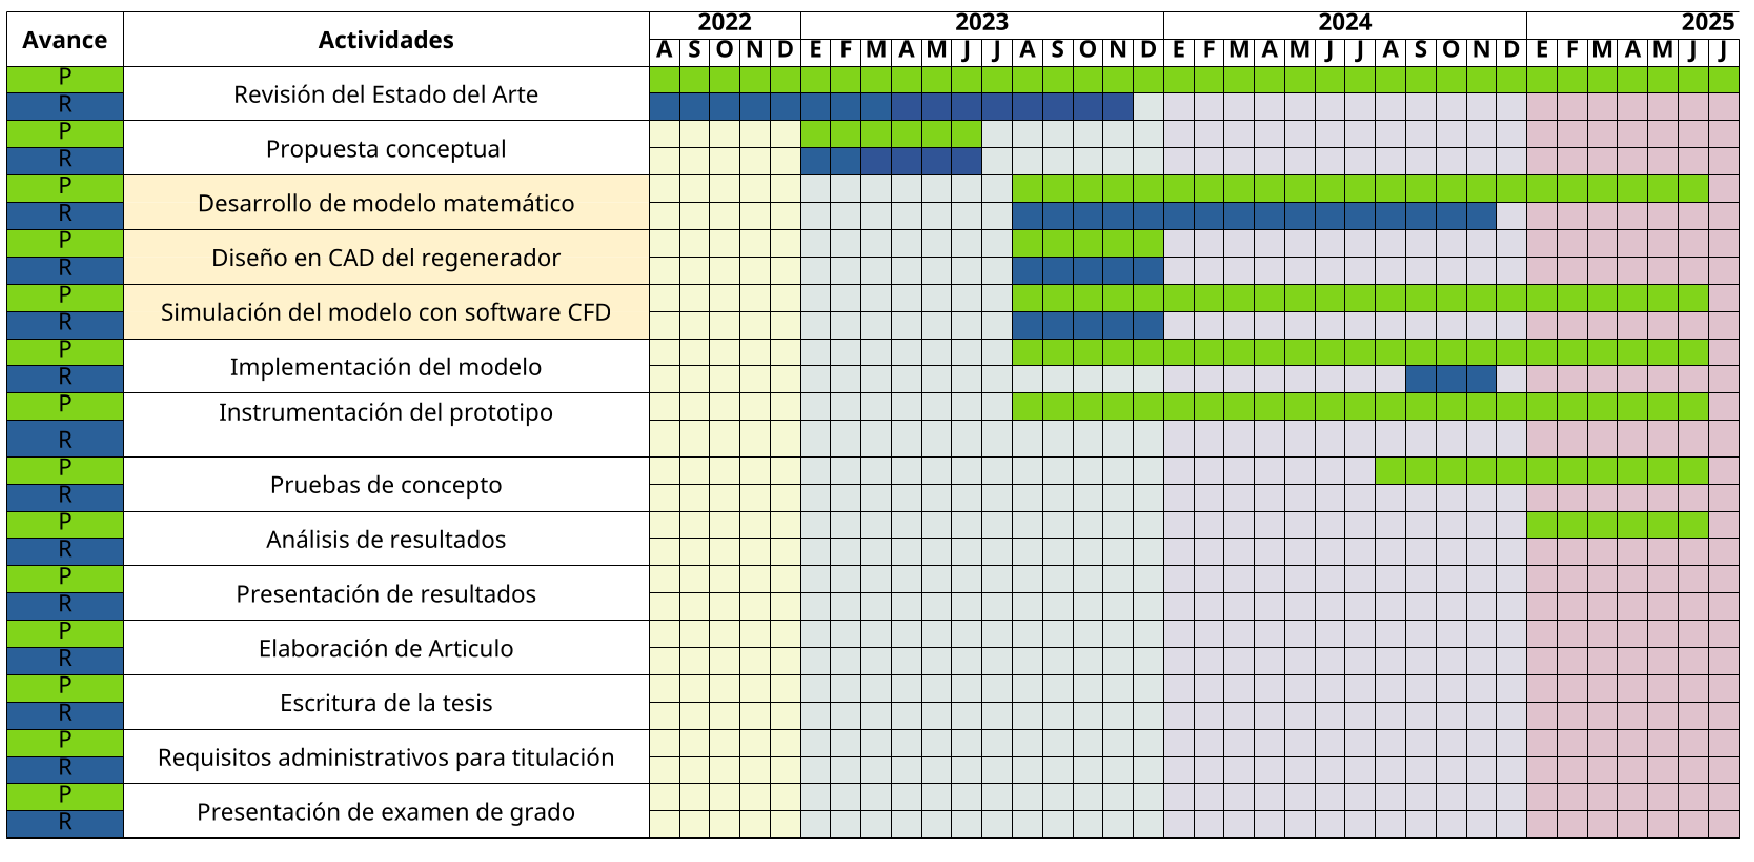
\includegraphics[scale=0.8]{crono_grama.pdf}
	\end{figure}
	\end{center}	
\end{landscape}

%%%%%%%%%%%%%%%%%%%%%%%%%%%%%%%%%%%%%%%%%
\newpage
\bibliographystyle{ieeetr}
\bibliography{referencias_5sem}

%\begin{landscape}
%	\appendix
%	\section{Velocidad de salida al regenerador}
	
%\end{landscape}

\end{document}
 